\documentclass{article} %this is an article
\usepackage[lmargin=.75in,rmargin=.75in,tmargin=1.in,bmargin=1in]{geometry} % setting margins
%\usepackage{tree-dvips}
\usepackage{tikz}  %makes crazy graphs
\usepackage{enumitem}
% \usetikzlibrary{snakes}
%\usepackage[flushleft]{threeparttable} %% makes notes for tables that wraps around width of table
%\usepackage{chronology}
\usepackage[round]{natbib}  %% beatiful bibliography
%\usepackage{wrapfig}
%\usepackage{longtable} %%multipage table
%\usepackage{qtree}
\usepackage{verbatim} %all kinds of shit
\usepackage{graphicx} %beautiful figures
%\usepackage{graphics}
%\usepackage{color}
%\usepackage{caption}
\usepackage{subcaption} %subcaption on the the subfigures
%\usepackage{multirow}
%\usepackage{sidecap}
%\usepackage{epstopdf}
\usepackage{amssymb} %beautiful math
\usepackage{amsmath,amssymb,amsfonts,amsthm,array} %beautiful math
\usepackage{amsthm}  %beautiful math
\usepackage{pgfplots}  %Normal distribution figure
\usepackage[colorlinks=true,linkcolor=red, citecolor=red]{hyperref} %sets my preferences for cross reference



\begin{document}
\begin{center}
  \textbf{Joao Rodrigues} \\
  \textbf{Economics 8185 - Computational Methods} \\
  \textbf{Homework 3c - Reiter (2009)} \\
  \textbf{Economics Department}
\end{center}
\section*{Model details}
Reiter (2009) had a innovative insight into Krusell \& Smith (1998) where he observed that agents responded to individual assets nonlinearly but to aggregate states linearly. He then decided to use perturbation methods around the steady state solution to solve for an equilibrium in a way that policies relate to individual assets nonlinearly but linearly to aggregate assets. He does this by solving an Aiyagari economy (steady state solution) and posing the problem as a linear rational expectations problem as in Sims (2001) \\
\\
Again, I solved both the exogenous and endogenous labor cases. This time, instead of using finite element method , I used collocation as in Reiter (2009). As before, I used Young (2010) in order to approximate the stationary distribution. I built a system as proposed in Reiter (2009) with $ns*na$ Euler equations, $ns*nx$ equations for the evolution of the distribution of assets, and an equation for the exogenous process (where na, nx, and ns are the sizes of grid on assets for individual policies, grid on assets for distribution, and number of idiosyncratic states). 
\section*{Computation}
After solved for the steady as in the Aiyagari exercise, then tok the transition matrix $\Pi$ built the following system of equations which can be written succintly as:
$$F(x',y',x,y,\eta,\epsilon) =
\left[ \begin{array}{cc} u_c(c(k_{i,\epsilon},\epsilon)) - \sum_{\epsilon'|\epsilon}u_c(c(k'(k_{i,\epsilon},\epsilon),\epsilon')) + \eta_{i,\epsilon} \\
    \lambda'(k,\epsilon) - \Pi\lambda(k,\epsilon)  \\
         \log( z') - \rho_z \log(z) - \omega_z \epsilon_z \end{array} \right]$$where $x=\{\theta_i\}_{i=1}^{na} $ represent states and $y=(\{\lambda_i\}_{i=1}^{nx},z)$ controls $\eta_{i,\epsilon}$ are exectational errors and $\epsilon$ are exogenous shocks. We can then put this system in Sims (2001) formulation:
     $$ \Gamma_0 X_{t} = \Gamma_1 X_{t-1} + \Psi \eta_t + \Pi \epsilon_t $$
where $X=(x,y)$ and solution have the form:
     $$X_t = A X_{t-1} + B\epsilon_t $$
     We need $\Gamma_0,\Gamma_0,\Psi,\Pi$ in order to solve the system. Following Sims (2001), we can define these matrices as:
     $$\Gamma_0 = -\frac{\partial F(X_t,X_{t-1},\eta_t,\epsilon_t)}{\partial X_t} \;\; \Gamma_1 = \frac{\partial F(X_t,X_{t-1},\eta_t,\epsilon_t)}{\partial X_{t-1}}, \;\; \Psi = \frac{\partial F(X_t,X_{t-1},\eta_t,\epsilon_t)}{\partial \eta_t}, \;\; \Pi = \frac{\partial F(X_t,X_{t-1},\eta_t,\epsilon_t)}{\partial \epsilon_t}$$
 \section*{results}
 Results in both endogenous and exogenous cases are quite similar. After solving Aiyagari, there is little work in adapting the code, to use Reiter's method on the solution coming out of Aiyagari. Below, are some plots of both exogenous and endogenous labor cases.     
\subsection*{Exogenous labor}
In the time series, we can see that in high productivity periods we have a lower mass of peple that are borrowing constrained. Further, the aggregate capital is higher under high productivity states and lower in lower productivity states. The stationary distribution is that of Aiyagari. 
\begin{figure}[h!]
  \centering
  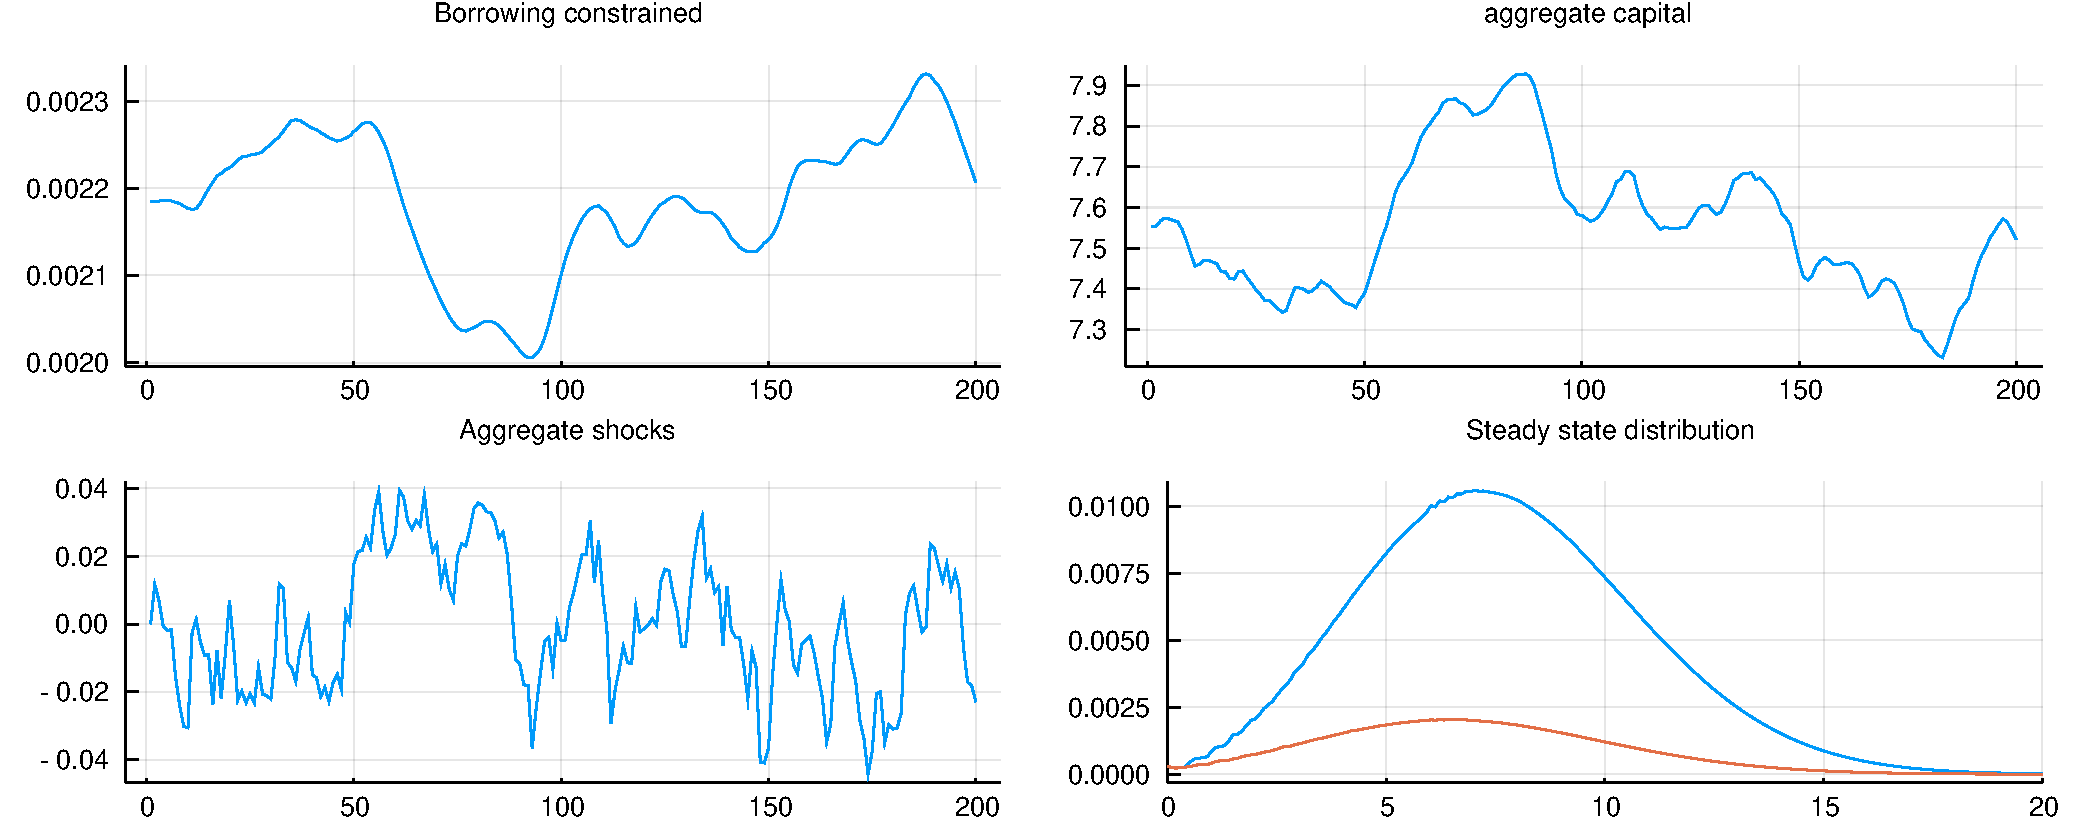
\includegraphics[width = 0.8\textwidth]{../exogenous/timeseries.pdf}
    \caption{Time series from a series of aggregate shocks and stationary distribution}
  \end{figure}
I also took the smallest and largest shock in my shock series and plotted the distributions in order to see the effect of aggregate shocks on distribution of asets (this is shown in figure 2). Note the spikes in the distribution, I suspect this might be due to the fact that we are fair away from steady state. Perhaps a method other than the histogram method delivers a distirbution of assets that is smoother. Regardless, note that these are almost 5\% shocks to productivity (5 times larger than productivity shocks in KS (1998)) and the distirbution of assets barely moves. This tells us that with the simple savings problem, aggregate states don't add a whole lot to a model without responses to aggregate shocks.
\begin{figure}[h!]
  \centering
  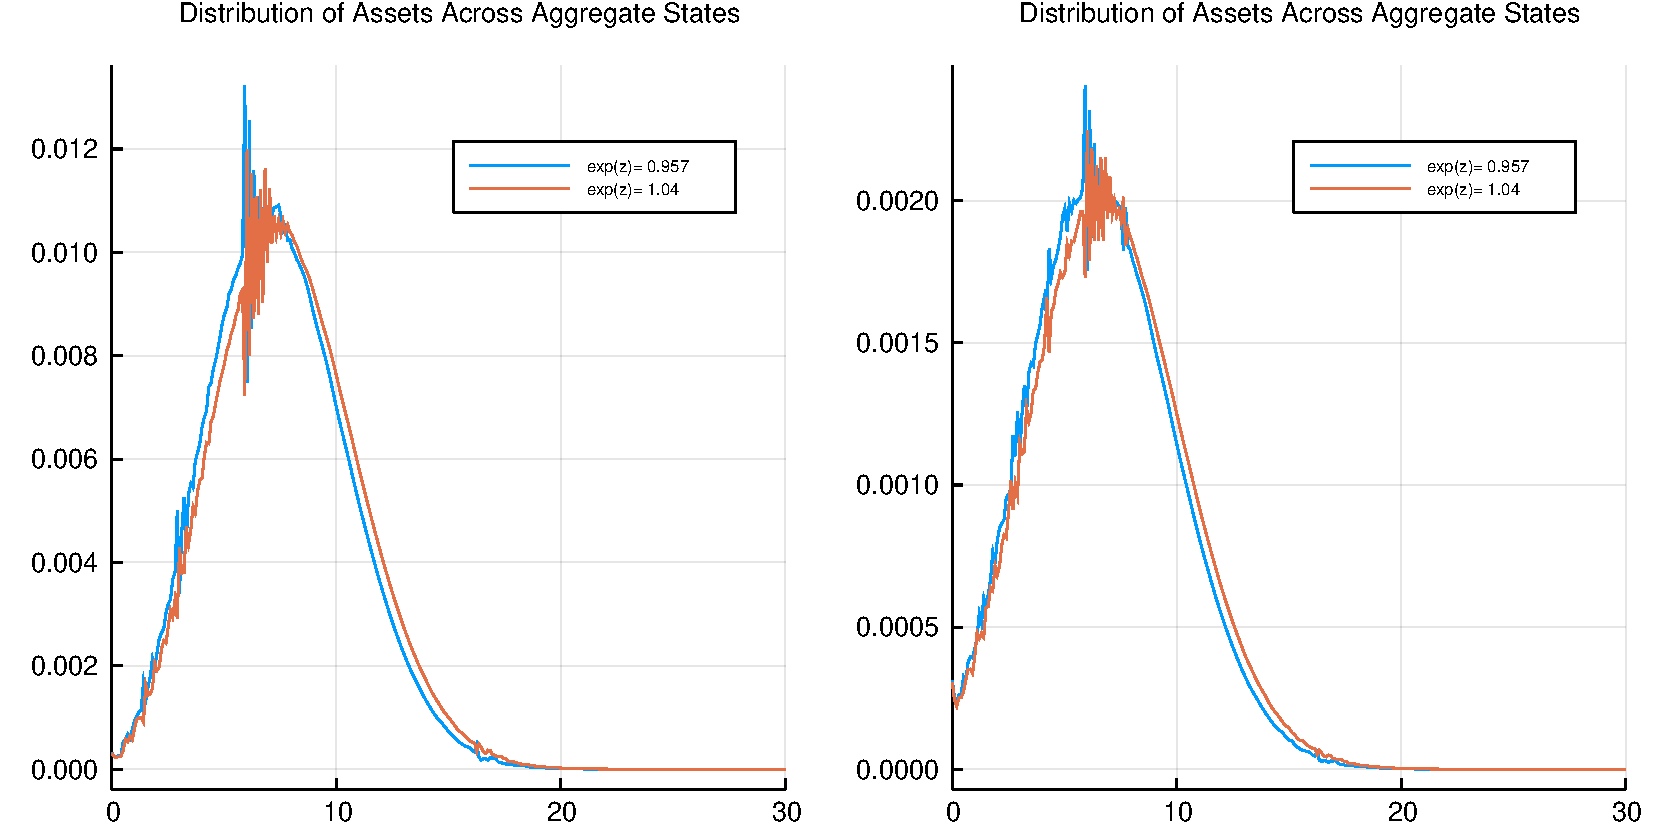
\includegraphics[width = 0.8\textwidth]{../exogenous/exodistribution.pdf}
    \caption{Time series from a series of aggregate shocks and stationary distribution}
  \end{figure}
\subsection*{Endogenous labor}
Below I plot the same figures for the case with elastic labor. As before, the distribution of assets has less skewness. And once again, response to aggregate shocks moves the distribution only slightly
\begin{figure}[h!]
  \centering
  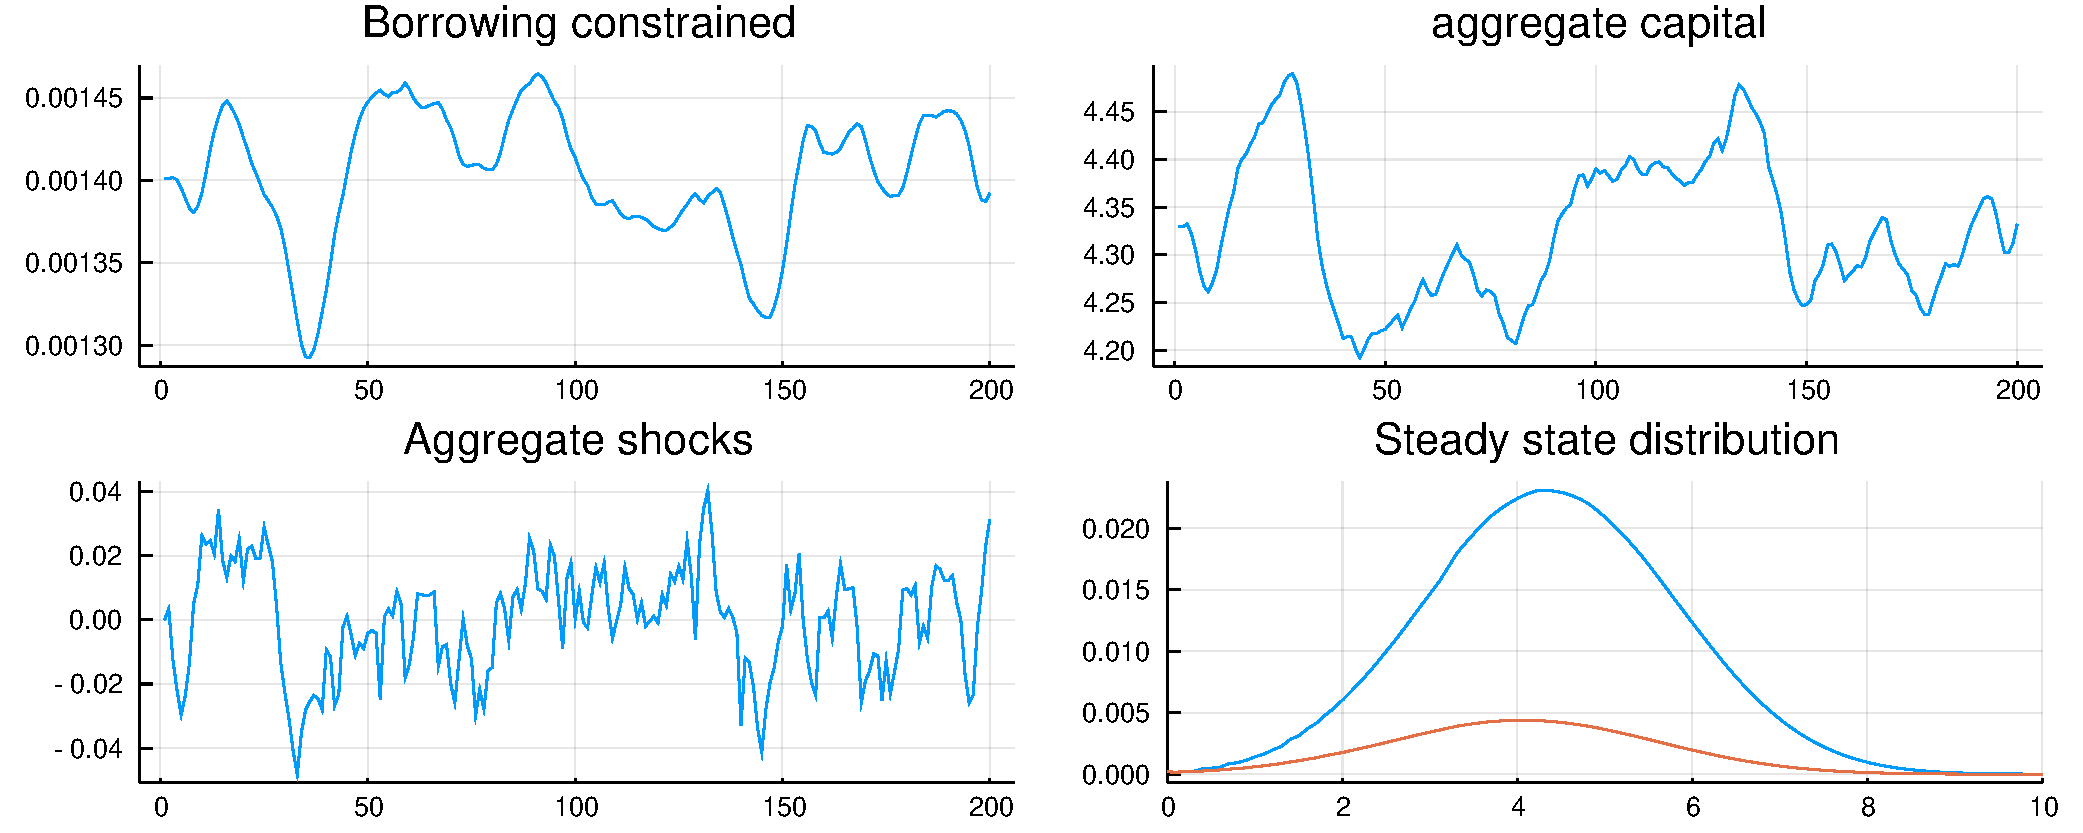
\includegraphics[width = 0.8\textwidth]{../endogenous_labor/timeseries.pdf}
    \caption{Time series from a series of aggregate shocks and stationary distribution}
  \end{figure}
\begin{figure}[h!]
  \centering
  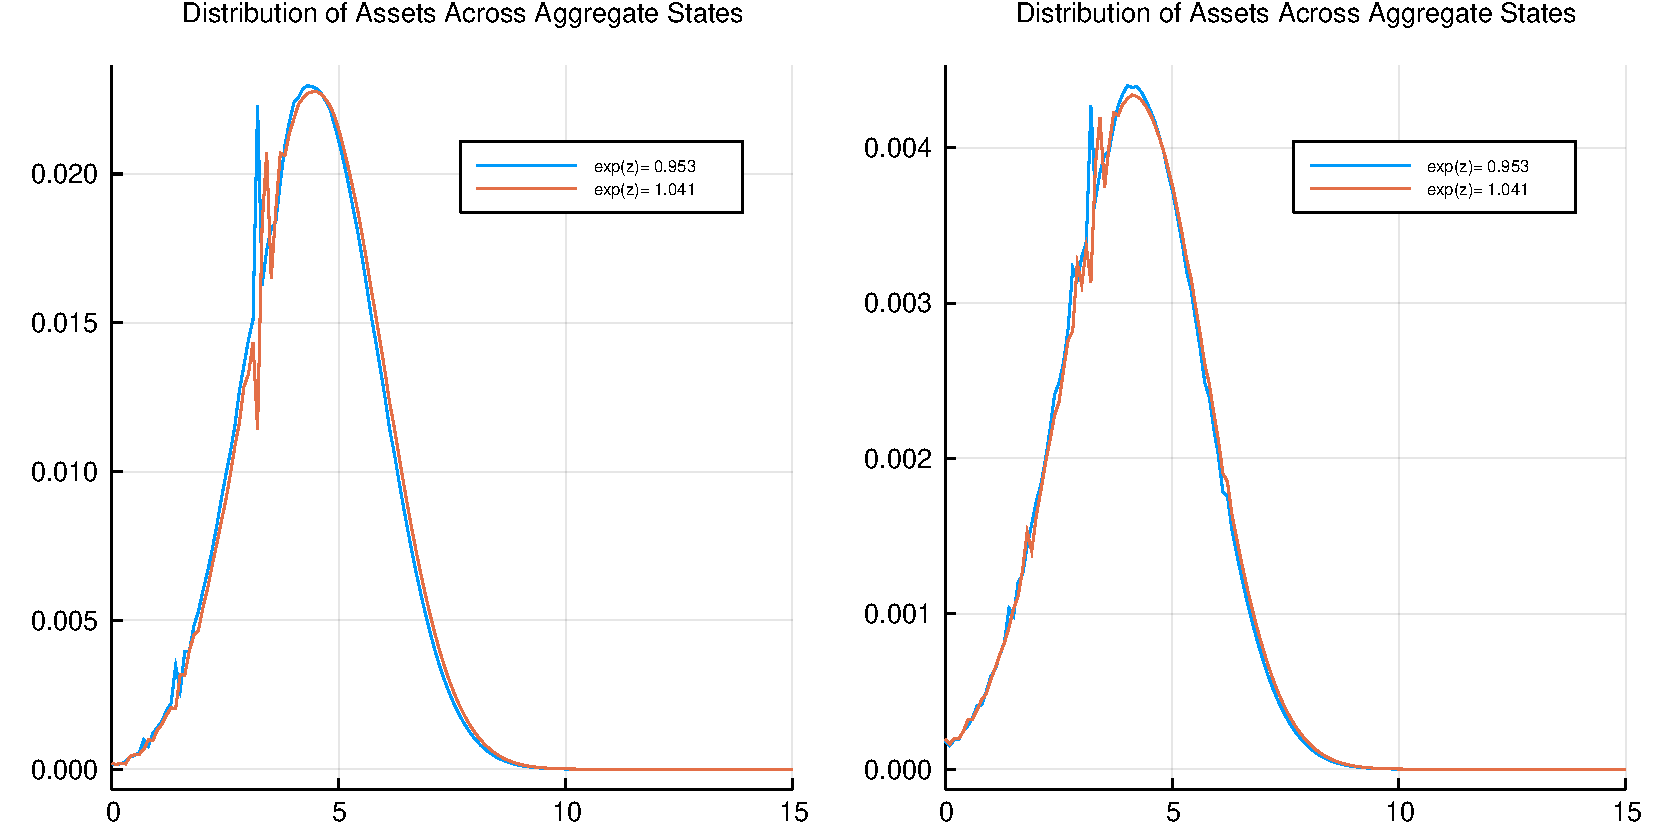
\includegraphics[width = 0.8\textwidth]{../endogenous_labor/enddistribution.pdf}
    \caption{Time series from a series of aggregate shocks and stationary distribution}
  \end{figure}


\end{document}
